% !TeX spellcheck = en_GB

%\section{Prior Work and Existing Solutions}
%\label{sec:background:network:priorwork}

\begin{comment}
	\begin{itemize}
		\item \parencite{Yang2006}
		\item \parencite{Celeda2012}
		\item \textcite{Pan2014} BACnet
			\begin{itemize}
				\item Anonmaly detection for BACnet fire alarm systems
				\item taps BACnet traffic via IP
				\item rule based learning (RIPPER)
				\item protection against common BACnet attack vectors
				\subitem who-is/who-has network probing
				\subitem write-property (take control over device)
				\subitem InitializedRoutingTable
				\subitem reinitialize devices
				\subitem application layer DoS
				\subitem flooding of network
			\end{itemize}
		
		\item \textcite{Eskin2002} algos for unsupervised anomaly detection in IDS
		\item \textcite{Leung2005} Unsupervised anomaly detection in IDS, proposed new algo \emph{pfMAFIA}
	\end{itemize}
\end{comment}

Despite being widely used and applied in \gls{ip} networks \parencite[cf.][pp.~201~ff.]{Northcutt2005}, \glspl{ids} seem to rather seldom utilized to monitor \glspl{bas}.
However, there are a few examples in literature where the principles of \glspl{ids} are applied to \gls{scada} and \gls{ics}.

One example of deploying anomaly in \gls{scada} networks is presented by \textcite{Yang2006}, with the base assumption that a security violation changes the system behaviour and that this change can be detected. They argue, that the repeatable and predictable nature of traffic in \gls{scada} networks make them an application field for anomaly detection based \glspl{ids}, opposed to rule based.
Further, they focus on inside threads where the attacker already has gained access and some knowledge about the targeted systems and possible vulnerabilities.
The proposed method is to use a \gls{aakr} model for anomaly detection to predict \emph{corrected} versions of their selected traffic features. Then the binary hypothesis technique \gls{sprt} is applied to determine if the observed sequence was likely to be generated by normal behaviour or not.
\textcite{Yang2006} show, that using \gls{aakr} with \gls{sprt} anomalies indicating malicious traffic can be identified in \gls{scada} networks.
However, they also note that it is crucial to monitor a large variety of system measurements and it is therefore an important task to carefully determine which variables are of value and which are not.

The threads in \gls{scada} networks, acknowledged by \textcite{Yang2006}, are also recognised by \textcite{Celeda2012}. They note, that not only \gls{scada} networks but also \gls{bas} provide more and more attack surfaces and exploiting those can have huge implications for companies and the society as a whole.
Further, security considerations in these networks are still highly underestimated, compared to \gls{ip} networks.
Consequently, \textcite{Celeda2012} argue that not only the intrinsic passive security of the protocols itself (cf. Section~\ref{sec:background:bas:knx:security}) needs to be increased, but intrusions and malicious behaviour have to be detected. Hence, they investigate possible applications and the advantages of flow-based monitoring (cf. Section~\ref{sec:background:network:netflow}) in \gls{bas}, specifically on the example of \gls{bac}.
The part of their research regarding flow analysis focuses on \gls{bac} over \gls{ip} and employs a simple volumetric approach (measuring the throughput) and calculates the entropy (cf. Section~\ref{sec:background:network:novelty:entropy}) of the flow data.
As a result \textcite{Celeda2012} were able to detect and identify several attacks and a bot net in \gls{bac} installations, based on flow data.

\begin{wrapfigure}{r}{0.6\textwidth}
	\vspace{-18pt}
	\centering
	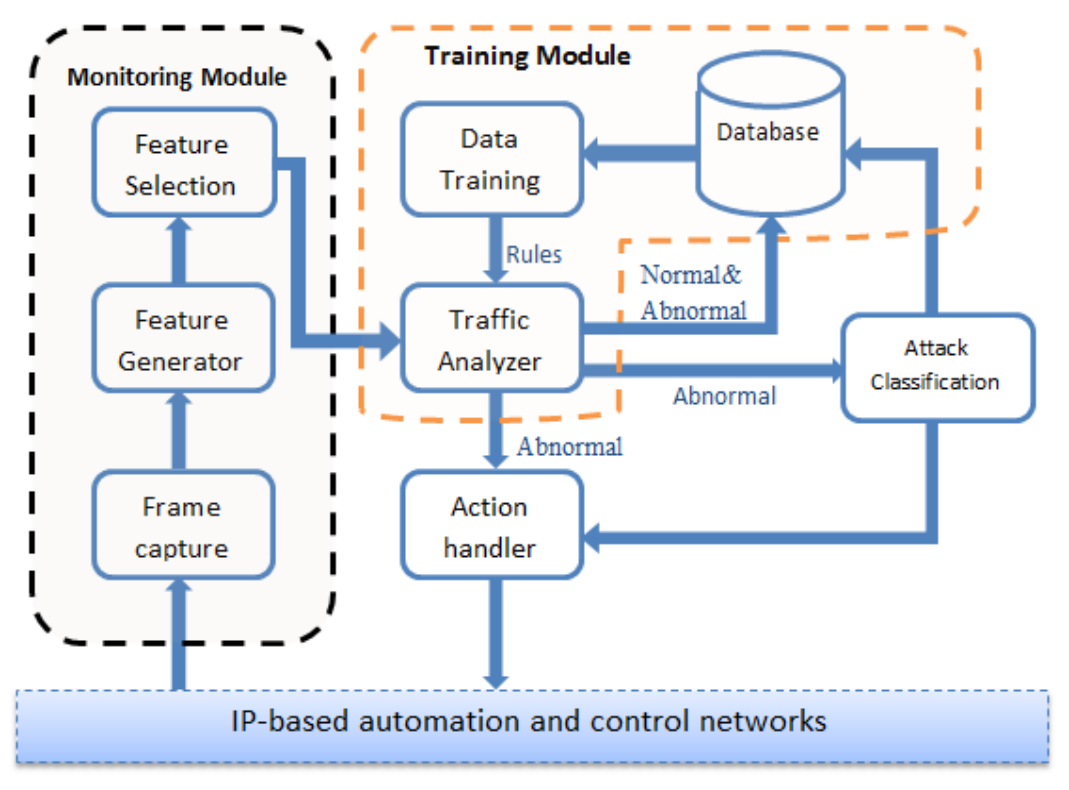
\includegraphics[width=0.6\textwidth,keepaspectratio]{figures/300-Pan2014-architecture.png}
	\caption[Anomaly detection framework architecture by Pan, Hairi, and Al-Nashif]{Anomaly detection framework architecture by \textcite{Pan2014}}
	\label{fig:background:prior-work:pan-architecture}
	\vspace{-20pt}
\end{wrapfigure}

Further investigations in \gls{bac} security are published by \textcite{Pan2014}. They present \enquote{a framework for a rule based anomaly detection} system in \gls{bas}, using \gls{bac} as example.
Similar to \textcite{Celeda2012}, \textcite{Pan2014} are relying on \gls{bac} over \gls{ip} to perform flow-analysis.
However, instead of employing rather simplistic measure to detect anomalies in flows, they build an elaborate framework around an inductive rule learning algorithm which also allows them to classification attacks.
This framework consists of four major modules: monitoring, training, attack classification, and action handling.
The monitoring module's basic function is to capture \gls{bac} packets, map the packet stream into a high dimensional feature space, select the most relevant features, and then store those into a database.
In the next step the stored feature vectors are fed into the training module, where during the training phase an inductive rule learning algorithm, called \glsfirst{ripper}, is applied.
The algorithm, first proposed by \textcite{Cohen1995}, is used in a two-class version on pre-labelled data and was applied by \textcite{Pan2014} to more than 7000 data points resulting in baseline model with 20 rules.
These rules are consequently used during the detection phase and applied on every flow-frame within a time window to improve the detection rate.
In case the rule framework detects an attack, the malicious packet flow is handed over to the attack classification module, which uses a decision table to classify the attack based on three attributes: the targeted protocol layer, the attack motivation, and the victim device.
The consideration of the targeted protocol layer accounts for different kinds of vulnerabilities within the protocol stack. \textcite{Pan2014} specifically focus on \gls{bac}'s \gls{apdu} and \gls{npdu}, which correspond to the application and network layer respectively.

Further, the attack classifier accounts for different attack motivations. This includes \emph{reconnaissance attacks}, which aim to collect information about the network and its traffic, \emph{device access attacks}, representing attempts to access devices without permission, and finally \emph{\gls{dos} attacks}, where the network and devices are saturated with useless commands to disturb normal operation.
The last attribute for attack classification is the targeted device, which uses domain knowledge about the network to assign roles to devices.
Finally, the classifications from the baseline model and the attack classifier are passed to the action handler module, which is designed to automatically trigger suitable mitigating measures. This includes extracting useful information, dropping packets or suspending connections based on a severity level of the attack, and producing an understandable alert message comprised of the prior gathered information.

All in all, \textcite{Pan2014} showed, that their framework is able to detect simulated attacks with a precision very close to 100\%. However, the test-bed they used was a fire detection system, which behaviour is purely deterministic and follows strict rules during normal operation.
Therefore, any discrepancy, indicating abnormal behaviour, can be easily detected.

% final words about limitations in Pan2014




